% Options for packages loaded elsewhere
\PassOptionsToPackage{unicode}{hyperref}
\PassOptionsToPackage{hyphens}{url}
%
\documentclass[
  man,floatsintext]{apa6}
\usepackage{amsmath,amssymb}
\usepackage{lmodern}
\usepackage{iftex}
\ifPDFTeX
  \usepackage[T1]{fontenc}
  \usepackage[utf8]{inputenc}
  \usepackage{textcomp} % provide euro and other symbols
\else % if luatex or xetex
  \usepackage{unicode-math}
  \defaultfontfeatures{Scale=MatchLowercase}
  \defaultfontfeatures[\rmfamily]{Ligatures=TeX,Scale=1}
\fi
% Use upquote if available, for straight quotes in verbatim environments
\IfFileExists{upquote.sty}{\usepackage{upquote}}{}
\IfFileExists{microtype.sty}{% use microtype if available
  \usepackage[]{microtype}
  \UseMicrotypeSet[protrusion]{basicmath} % disable protrusion for tt fonts
}{}
\makeatletter
\@ifundefined{KOMAClassName}{% if non-KOMA class
  \IfFileExists{parskip.sty}{%
    \usepackage{parskip}
  }{% else
    \setlength{\parindent}{0pt}
    \setlength{\parskip}{6pt plus 2pt minus 1pt}}
}{% if KOMA class
  \KOMAoptions{parskip=half}}
\makeatother
\usepackage{xcolor}
\usepackage{longtable,booktabs,array}
\usepackage{calc} % for calculating minipage widths
% Correct order of tables after \paragraph or \subparagraph
\usepackage{etoolbox}
\makeatletter
\patchcmd\longtable{\par}{\if@noskipsec\mbox{}\fi\par}{}{}
\makeatother
% Allow footnotes in longtable head/foot
\IfFileExists{footnotehyper.sty}{\usepackage{footnotehyper}}{\usepackage{footnote}}
\makesavenoteenv{longtable}
\usepackage{graphicx}
\makeatletter
\def\maxwidth{\ifdim\Gin@nat@width>\linewidth\linewidth\else\Gin@nat@width\fi}
\def\maxheight{\ifdim\Gin@nat@height>\textheight\textheight\else\Gin@nat@height\fi}
\makeatother
% Scale images if necessary, so that they will not overflow the page
% margins by default, and it is still possible to overwrite the defaults
% using explicit options in \includegraphics[width, height, ...]{}
\setkeys{Gin}{width=\maxwidth,height=\maxheight,keepaspectratio}
% Set default figure placement to htbp
\makeatletter
\def\fps@figure{htbp}
\makeatother
\setlength{\emergencystretch}{3em} % prevent overfull lines
\providecommand{\tightlist}{%
  \setlength{\itemsep}{0pt}\setlength{\parskip}{0pt}}
\setcounter{secnumdepth}{-\maxdimen} % remove section numbering
% Make \paragraph and \subparagraph free-standing
\ifx\paragraph\undefined\else
  \let\oldparagraph\paragraph
  \renewcommand{\paragraph}[1]{\oldparagraph{#1}\mbox{}}
\fi
\ifx\subparagraph\undefined\else
  \let\oldsubparagraph\subparagraph
  \renewcommand{\subparagraph}[1]{\oldsubparagraph{#1}\mbox{}}
\fi
\newlength{\cslhangindent}
\setlength{\cslhangindent}{1.5em}
\newlength{\csllabelwidth}
\setlength{\csllabelwidth}{3em}
\newlength{\cslentryspacingunit} % times entry-spacing
\setlength{\cslentryspacingunit}{\parskip}
\newenvironment{CSLReferences}[2] % #1 hanging-ident, #2 entry spacing
 {% don't indent paragraphs
  \setlength{\parindent}{0pt}
  % turn on hanging indent if param 1 is 1
  \ifodd #1
  \let\oldpar\par
  \def\par{\hangindent=\cslhangindent\oldpar}
  \fi
  % set entry spacing
  \setlength{\parskip}{#2\cslentryspacingunit}
 }%
 {}
\usepackage{calc}
\newcommand{\CSLBlock}[1]{#1\hfill\break}
\newcommand{\CSLLeftMargin}[1]{\parbox[t]{\csllabelwidth}{#1}}
\newcommand{\CSLRightInline}[1]{\parbox[t]{\linewidth - \csllabelwidth}{#1}\break}
\newcommand{\CSLIndent}[1]{\hspace{\cslhangindent}#1}
\ifLuaTeX
\usepackage[bidi=basic]{babel}
\else
\usepackage[bidi=default]{babel}
\fi
\babelprovide[main,import]{english}
% get rid of language-specific shorthands (see #6817):
\let\LanguageShortHands\languageshorthands
\def\languageshorthands#1{}
% Manuscript styling
\usepackage{upgreek}
\captionsetup{font=singlespacing,justification=justified}

% Table formatting
\usepackage{longtable}
\usepackage{lscape}
% \usepackage[counterclockwise]{rotating}   % Landscape page setup for large tables
\usepackage{multirow}		% Table styling
\usepackage{tabularx}		% Control Column width
\usepackage[flushleft]{threeparttable}	% Allows for three part tables with a specified notes section
\usepackage{threeparttablex}            % Lets threeparttable work with longtable

% Create new environments so endfloat can handle them
% \newenvironment{ltable}
%   {\begin{landscape}\centering\begin{threeparttable}}
%   {\end{threeparttable}\end{landscape}}
\newenvironment{lltable}{\begin{landscape}\centering\begin{ThreePartTable}}{\end{ThreePartTable}\end{landscape}}

% Enables adjusting longtable caption width to table width
% Solution found at http://golatex.de/longtable-mit-caption-so-breit-wie-die-tabelle-t15767.html
\makeatletter
\newcommand\LastLTentrywidth{1em}
\newlength\longtablewidth
\setlength{\longtablewidth}{1in}
\newcommand{\getlongtablewidth}{\begingroup \ifcsname LT@\roman{LT@tables}\endcsname \global\longtablewidth=0pt \renewcommand{\LT@entry}[2]{\global\advance\longtablewidth by ##2\relax\gdef\LastLTentrywidth{##2}}\@nameuse{LT@\roman{LT@tables}} \fi \endgroup}

% \setlength{\parindent}{0.5in}
% \setlength{\parskip}{0pt plus 0pt minus 0pt}

% Overwrite redefinition of paragraph and subparagraph by the default LaTeX template
% See https://github.com/crsh/papaja/issues/292
\makeatletter
\renewcommand{\paragraph}{\@startsection{paragraph}{4}{\parindent}%
  {0\baselineskip \@plus 0.2ex \@minus 0.2ex}%
  {-1em}%
  {\normalfont\normalsize\bfseries\itshape\typesectitle}}

\renewcommand{\subparagraph}[1]{\@startsection{subparagraph}{5}{1em}%
  {0\baselineskip \@plus 0.2ex \@minus 0.2ex}%
  {-\z@\relax}%
  {\normalfont\normalsize\itshape\hspace{\parindent}{#1}\textit{\addperi}}{\relax}}
\makeatother

% \usepackage{etoolbox}
\makeatletter
\patchcmd{\HyOrg@maketitle}
  {\section{\normalfont\normalsize\abstractname}}
  {\section*{\normalfont\normalsize\abstractname}}
  {}{\typeout{Failed to patch abstract.}}
\patchcmd{\HyOrg@maketitle}
  {\section{\protect\normalfont{\@title}}}
  {\section*{\protect\normalfont{\@title}}}
  {}{\typeout{Failed to patch title.}}
\makeatother

\usepackage{xpatch}
\makeatletter
\xapptocmd\appendix
  {\xapptocmd\section
    {\addcontentsline{toc}{section}{\appendixname\ifoneappendix\else~\theappendix\fi\\: #1}}
    {}{\InnerPatchFailed}%
  }
{}{\PatchFailed}
\keywords{Diabetes, access to care, inflammation, health, Mexico, China\newline\indent Word count: X (this cannot easily be done automatically, we can also just leave it out)}
\usepackage{csquotes}
\usepackage[titles]{tocloft}
\cftpagenumbersoff{figure}
\renewcommand{\cftfigpresnum}{\itshape\figurename\enspace}
\renewcommand{\cftfigaftersnum}{.\space}
\setlength{\cftfigindent}{0pt}
\setlength{\cftafterloftitleskip}{0pt}
\settowidth{\cftfignumwidth}{Figure 10.\qquad}
\cftpagenumbersoff{table}
\renewcommand{\cfttabpresnum}{\itshape\tablename\enspace}
\renewcommand{\cfttabaftersnum}{.\space}
\setlength{\cfttabindent}{0pt}
\setlength{\cftafterloftitleskip}{0pt}
\settowidth{\cfttabnumwidth}{Table 10.\qquad}
\ifLuaTeX
  \usepackage{selnolig}  % disable illegal ligatures
\fi
\IfFileExists{bookmark.sty}{\usepackage{bookmark}}{\usepackage{hyperref}}
\IfFileExists{xurl.sty}{\usepackage{xurl}}{} % add URL line breaks if available
\urlstyle{same} % disable monospaced font for URLs
\hypersetup{
  pdftitle={Relations between Inflammation and Access to care, Treatment, and Diabetes in a repesentative population of Mexico or Relations between inflammation and access to care and treatment among Mexicans 50 years of age or older with diabetes in Mexico},
  pdfauthor={Dominik Grätz1, Rachel Miller-Moudgil1, Amber Somarriba1, Brittany Spinner1, \& Tian Walker1},
  pdflang={en-EN},
  pdfkeywords={Diabetes, access to care, inflammation, health, Mexico, China},
  hidelinks,
  pdfcreator={LaTeX via pandoc}}

\title{Relations between Inflammation and Access to care, Treatment, and Diabetes in a repesentative population of Mexico or Relations between inflammation and access to care and treatment among Mexicans 50 years of age or older with diabetes in Mexico}
\author{Dominik Grätz\textsuperscript{1}, Rachel Miller-Moudgil\textsuperscript{1}, Amber Somarriba\textsuperscript{1}, Brittany Spinner\textsuperscript{1}, \& Tian Walker\textsuperscript{1}}
\date{}


<<<<<<< Updated upstream
\shorttitle{Inflammation, Access to care, and Treatment among those with Diabetes in Mexico.}
=======
\shorttitle{Inflammation, access to care and Diabetes in Mexico.}
>>>>>>> Stashed changes

\authornote{List of group members ordered by alphabet.}

\affiliation{\vspace{0.5cm}\textsuperscript{1} University of Oregon}

\abstract{%
\emph{Background.} Background goes here. \emph{Methods.} Methods go here. \emph{Results.} Results here. \emph{Conclusions.} Conclusions here.
}



\begin{document}
\maketitle

\begin{figure}[H]
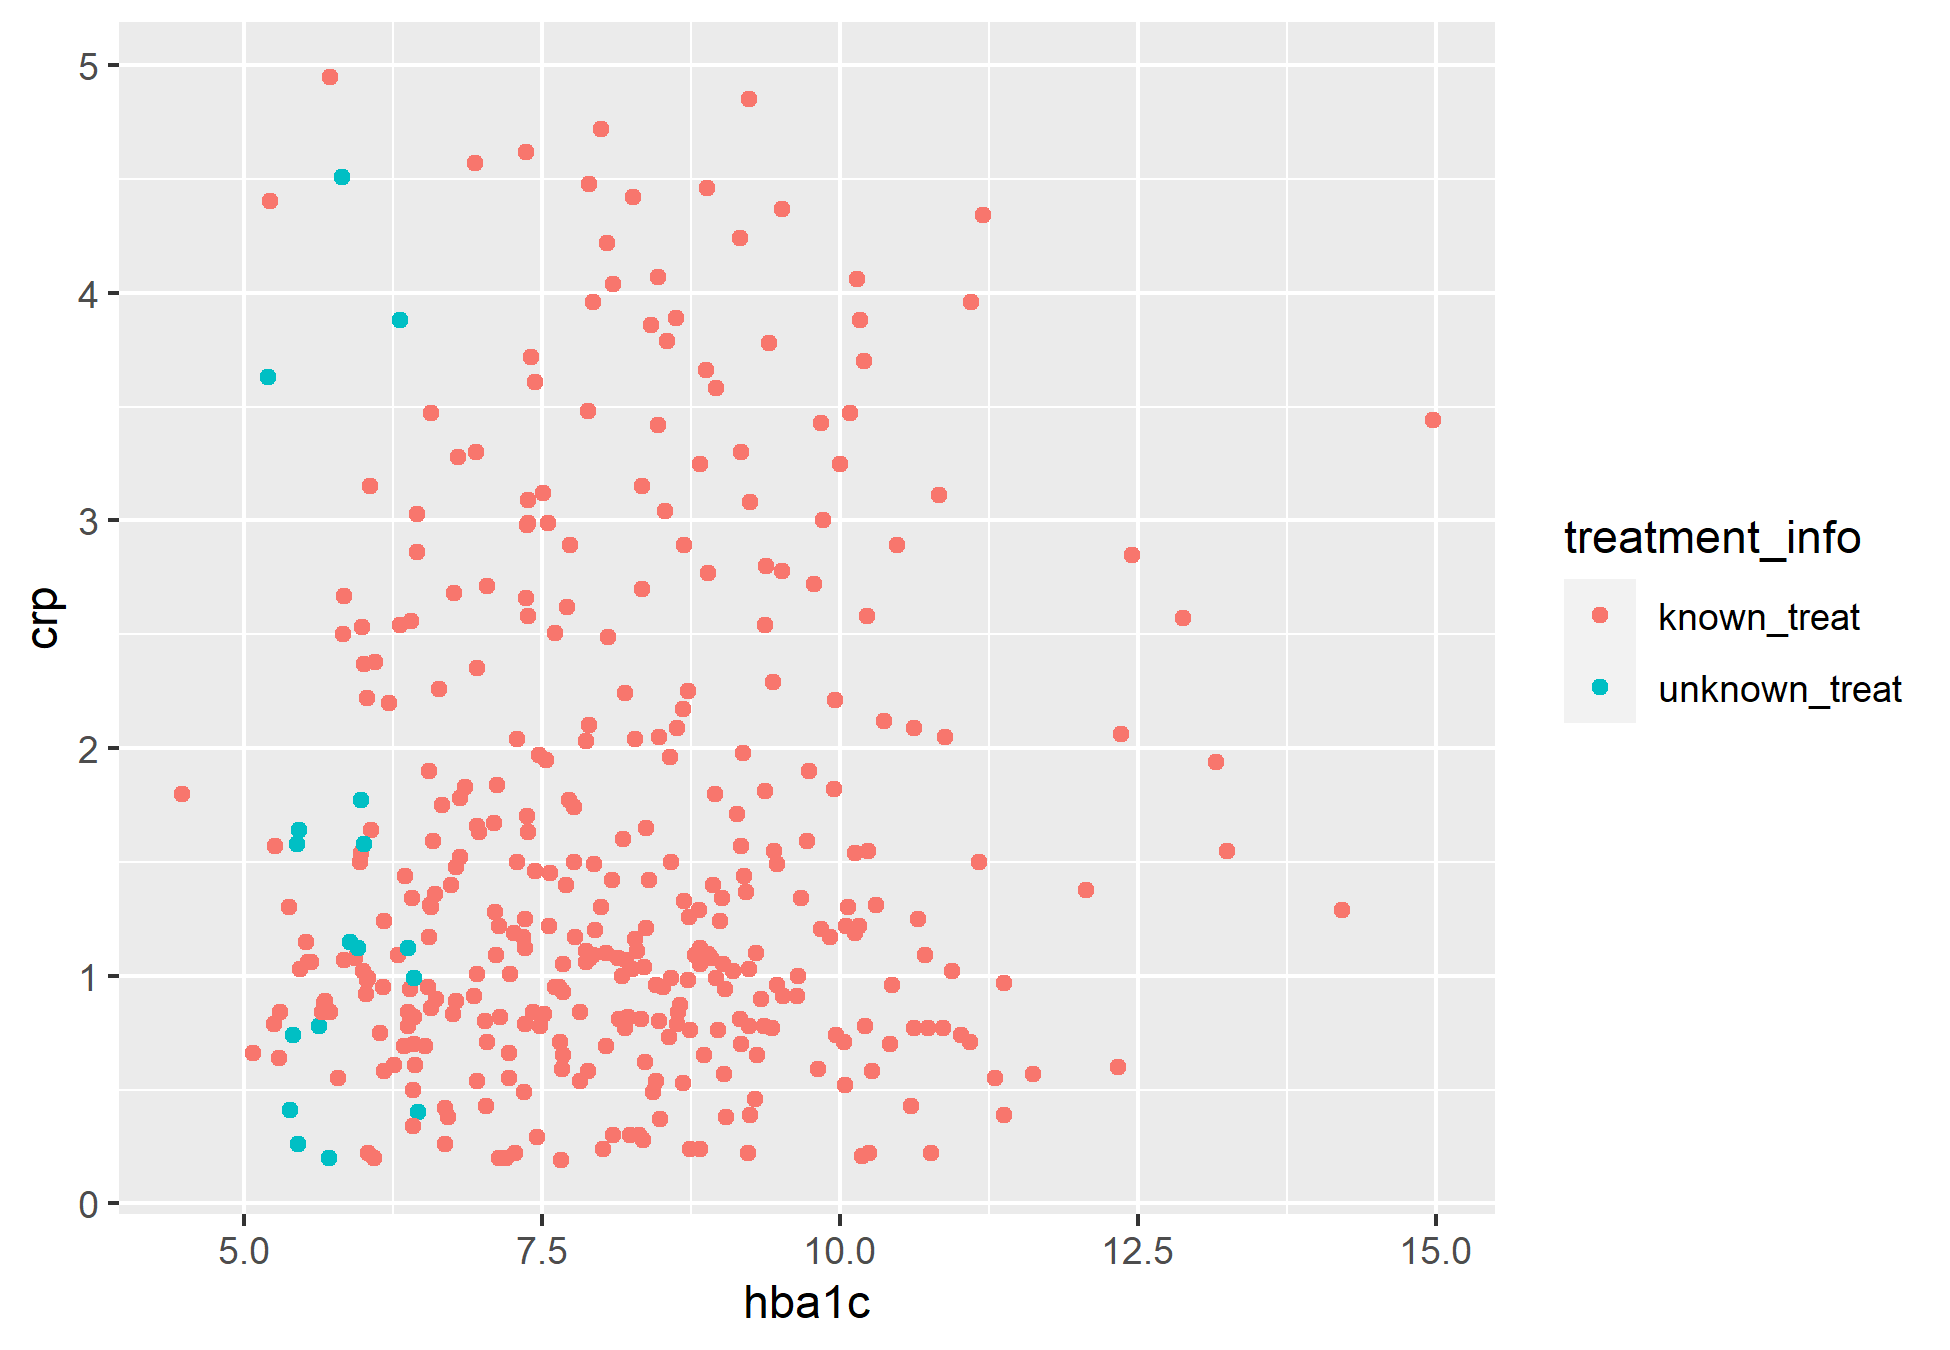
\includegraphics{NEW_Final_Groupof5_files/figure-latex/data-cleaning-tian2-1} \caption{Figure \ref{fig:data-cleaning-tian2} caption goes here.}\label{fig:data-cleaning-tian2}
\end{figure}



Here I point the reader to figure \ref{fig:data-cleaning-tian2}.

\begin{figure}[H]
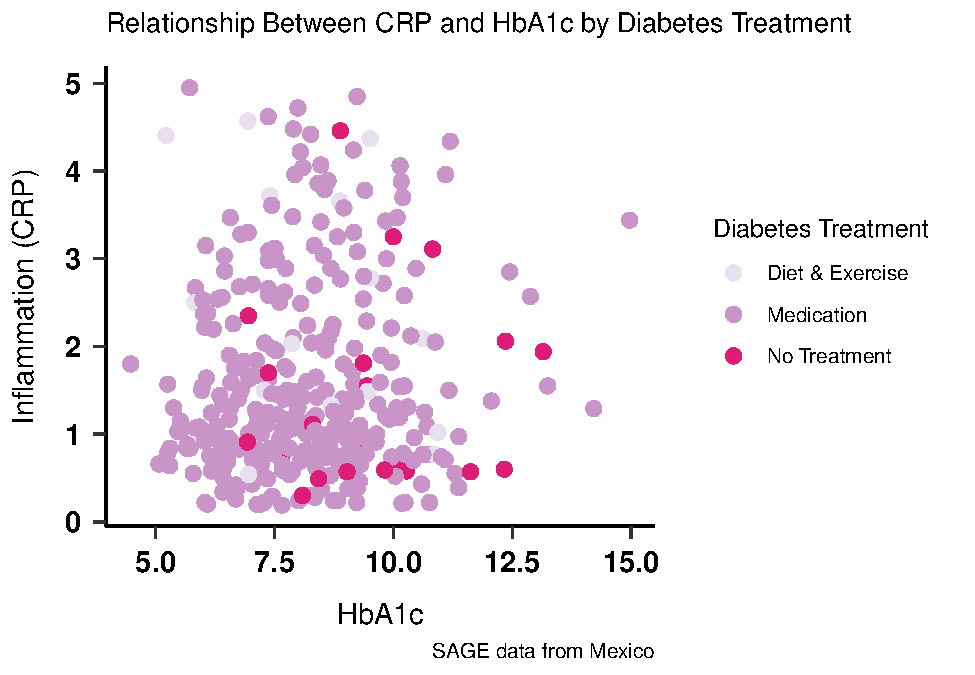
\includegraphics{NEW_Final_Groupof5_files/figure-latex/fig1-1} \caption{This is the caption of figure \ref{fig:fig1}.}\label{fig:fig1}
\end{figure}



Here, I want to point the reader to Figure \ref{fig:fig1}.

\begin{figure}[H]
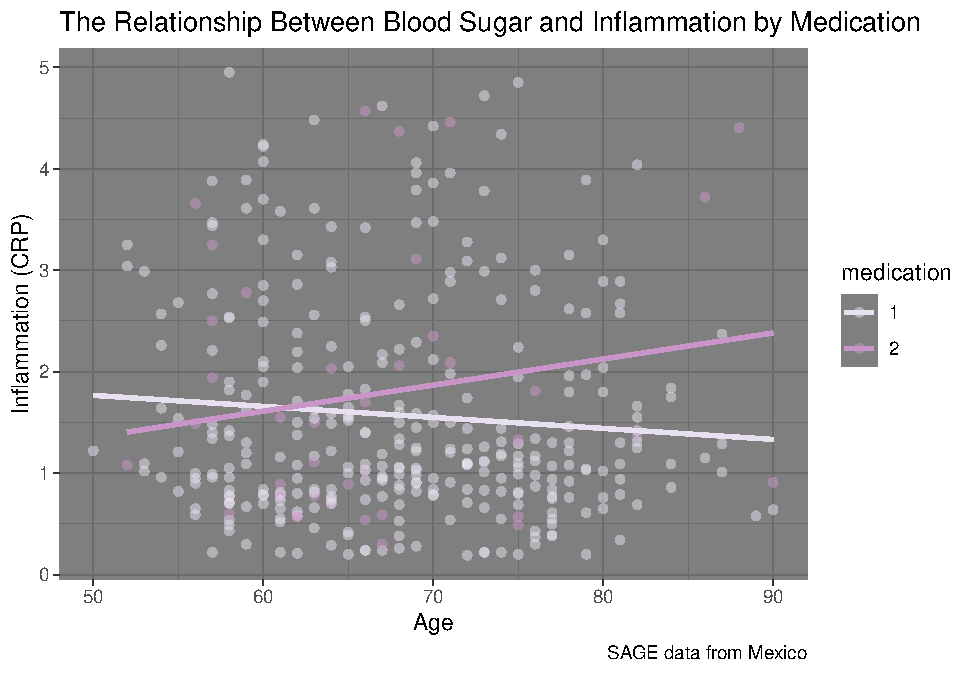
\includegraphics{NEW_Final_Groupof5_files/figure-latex/fig2-1} \caption{This is the caption this figure.}\label{fig:fig2}
\end{figure}



Here, I want to point the reader to Figure \ref{fig:fig2}.

\begin{figure}[H]
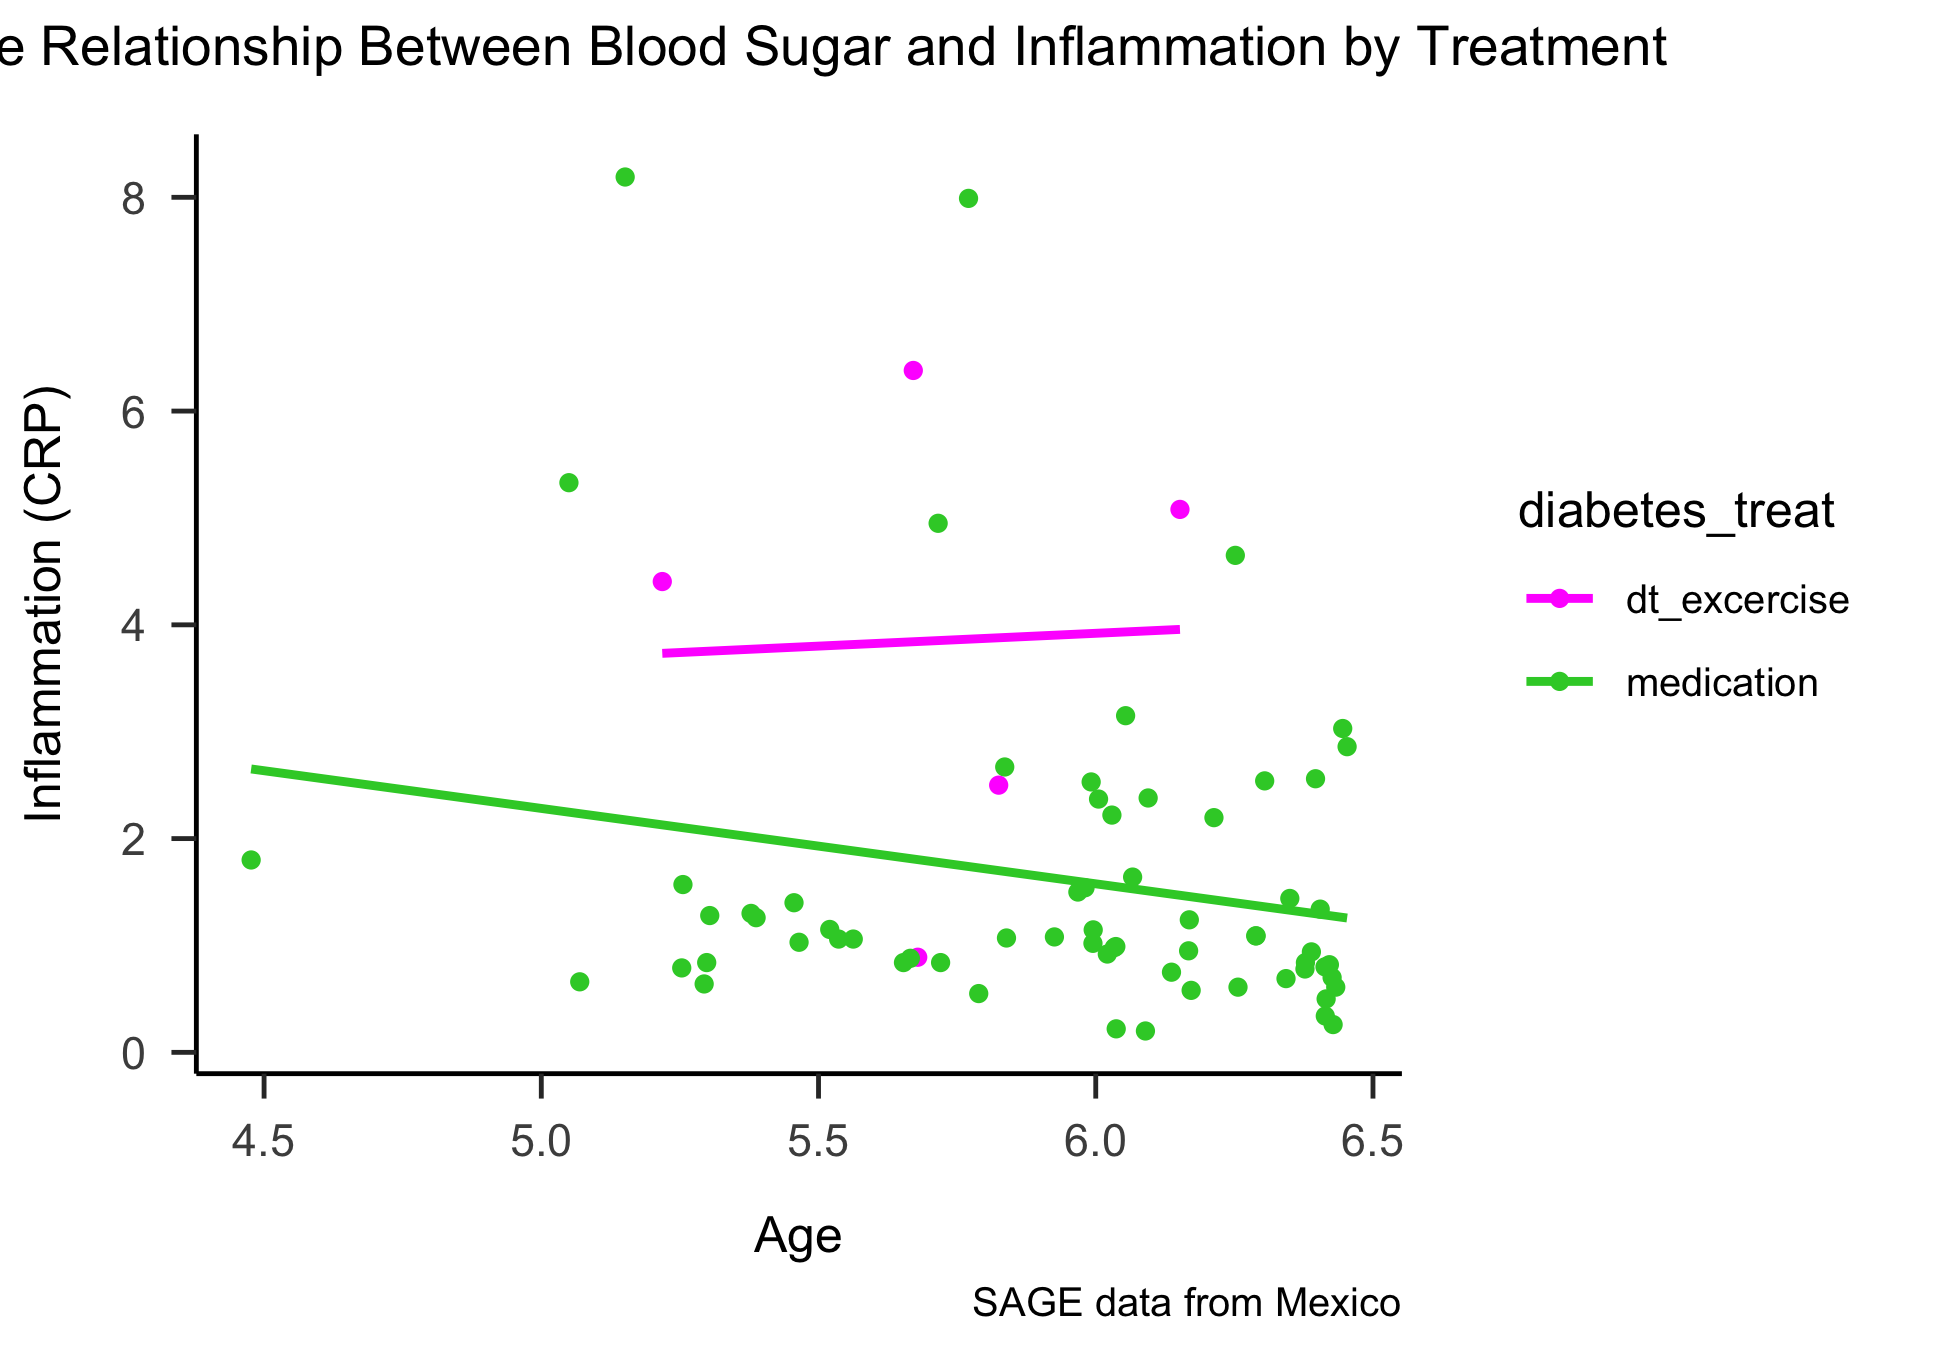
\includegraphics{NEW_Final_Groupof5_files/figure-latex/fig3-1} \caption{This is the caption of figure \ref{fig:fig3}.}\label{fig:fig3}
\end{figure}



Here, I want to point the reader to Figure \ref{fig:fig3}.

\begin{table}[tbp]

\begin{center}
\begin{threeparttable}

\caption{\label{tab:regtab1}Effect of Medication on CRP, controlling for Age. }

\begin{tabular}{lllllll}
\toprule
Predictor & \multicolumn{1}{c}{$b$} & \multicolumn{1}{c}{95\% CI} & \multicolumn{1}{c}{$t$} & \multicolumn{1}{c}{$\mathit{df}$} & \multicolumn{1}{c}{$p$} & \multicolumn{1}{c}{predictor}\\
\midrule
Intercept & 2.00 & {}[1.06, 2.94] & 4.18 & 354 & < .001 & Intercept\\
Age & -0.01 & {}[-0.02, 0.01] & -0.91 & 354 & .362 & Age\\
Medication2 & 0.20 & {}[-0.17, 0.56] & 1.07 & 354 & .284 & Medication\\
\bottomrule
\addlinespace
\end{tabular}

\begin{tablenotes}[para]
\normalsize{\textit{Note.} Model fit: $F$(2, 354) = 1.06, $p$ = 0.35, $R^2$ = 0.01.}
\end{tablenotes}

\end{threeparttable}
\end{center}

\end{table}

Demo of inline code usage. We found that this regression model (Table \ref{tab:regtab1}) using 357 participants was not significant \(F\)(2, 354) = 1.06, \(p\) = 0.35 with \(R^2\) = 0.01. The regression coefficient for age was \(b_{age}\) = -0.01 (\(SE\) = 0.01, \(p\) = 0.36), and for use of medication \(b_{medication}\) = 0.20 (\(SE\) = 0.18, \(p\) = 0.28).

\newpage

\begin{table}[tbp]

\begin{center}
\begin{threeparttable}

\caption{\label{tab:RQ2}Effect of Diet and Exercise on CRP, controlling for Age.}

\begin{tabular}{lllllll}
\toprule
Predictor & \multicolumn{1}{c}{$b$} & \multicolumn{1}{c}{95\% CI} & \multicolumn{1}{c}{$t$} & \multicolumn{1}{c}{$\mathit{df}$} & \multicolumn{1}{c}{$p$} & \multicolumn{1}{c}{predictor}\\
\midrule
Intercept & 2.10 & {}[1.17, 3.04] & 4.43 & 354 & < .001 & Intercept\\
Age & -0.01 & {}[-0.02, 0.01] & -0.83 & 354 & .408 & Age\\
Dt exrcse2 & -0.25 & {}[-0.47, -0.02] & -2.11 & 354 & .036 & Diet and Exercise\\
\bottomrule
\addlinespace
\end{tabular}

\begin{tablenotes}[para]
\normalsize{\textit{Note.} Model fit: $F$(2, 354) = 2.71, $p$ = 0.07, $R^2$ = 0.02.}
\end{tablenotes}

\end{threeparttable}
\end{center}

\end{table}

Demo of inline code usage. We found that this regression model (Table \ref{tab:RQ2}) using 354 participants was not significant \(F\)(2, 354) = 2.70, \(p\) = 0.07 with \(R^2\) = 0.02. The regression coefficient for age was \(b_{age}\) = -0.01 (\(SE\) = 0.01, \(p\) = 0.41), and for diet and exercise \(b_{Diet}\) = -0.24 (\(SE\) = 0.12, \(p\) \textless{} 0.05).
<<<<<<< Updated upstream

\begin{verbatim}
## # A tibble: 171 x 2
##    `RQ4df$access` `RQ4df$crp2`
##    <fct>          <fct>       
##  1 No             high        
##  2 No             low         
##  3 Yes            low         
##  4 No             low         
##  5 No             low         
##  6 No             low         
##  7 Yes            low         
##  8 Yes            low         
##  9 No             low         
## 10 No             high        
## # ... with 161 more rows
\end{verbatim}

\begin{verbatim}
## 
##  Pearson's Chi-squared test with Yates' continuity correction
## 
## data:  RQ4df$access and RQ4df$crp2
## X-squared = 0.51779, df = 1, p-value = 0.4718
\end{verbatim}

\begin{verbatim}
##             RQ4df$crp2
## RQ4df$access      low     high
##          Yes 67.26316 13.73684
##          No  74.73684 15.26316
\end{verbatim}

\begin{verbatim}
##             RQ4df$crp2
## RQ4df$access low high
##          Yes  65   16
##          No   77   13
\end{verbatim}

\begin{verbatim}
## 
##       Yes        No 
## 0.4736842 0.5263158
\end{verbatim}

\begin{verbatim}
## 
##       low      high 
## 0.8304094 0.1695906
\end{verbatim}

\begin{figure}[H]
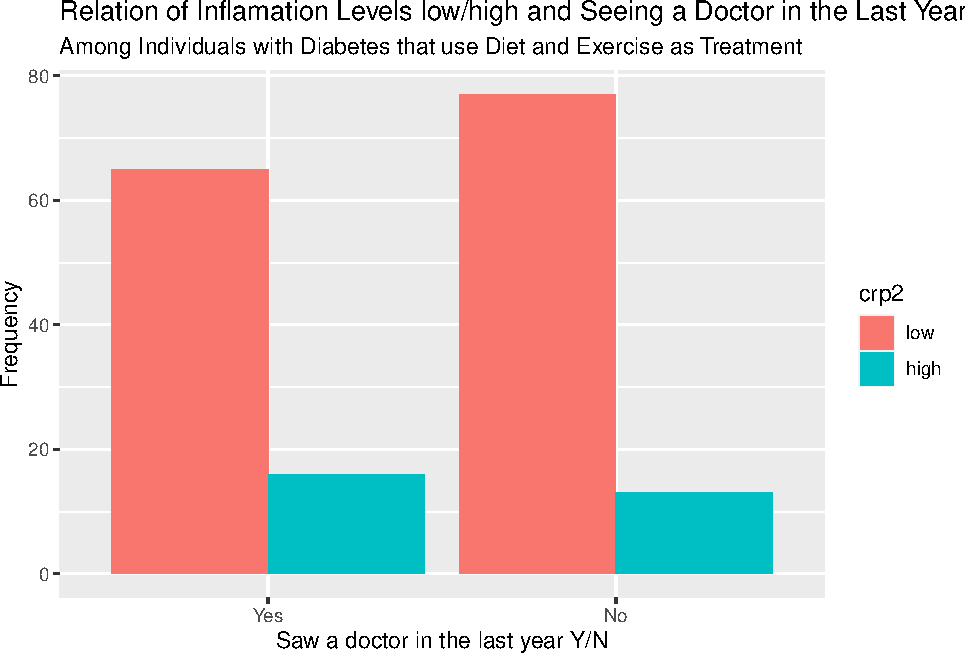
\includegraphics{NEW_Final_Groupof5_files/figure-latex/unnamed-chunk-1-1} \caption{ }\label{fig:unnamed-chunk-1}
\end{figure}

\begin{verbatim}
## 
##  Chi-squared test for given probabilities
## 
## data:  table(data$sex)
## X-squared = 44.596, df = 1, p-value = 2.422e-11
\end{verbatim}
=======
>>>>>>> Stashed changes

\begin{figure}[H]
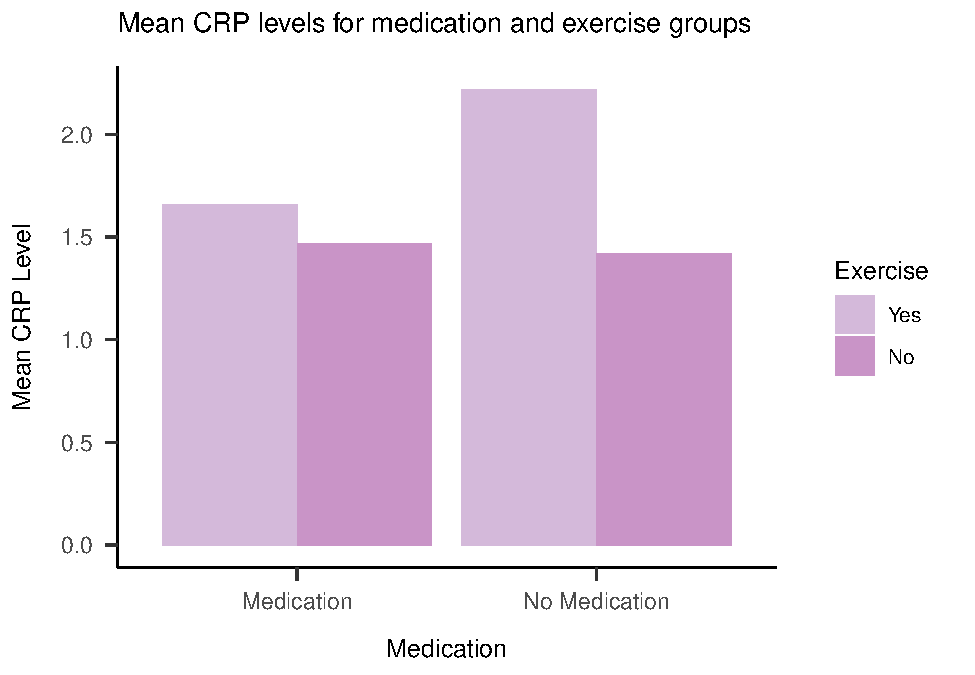
\includegraphics{NEW_Final_Groupof5_files/figure-latex/tableofcrpmedicationandexercise-1} \caption{Caption for Figure \ref{fig:tableofcrpmedicationandexercise} goes here.}\label{fig:tableofcrpmedicationandexercise}
\end{figure}



Here I reference figure \ref{fig:tableofcrpmedicationandexercise}.

\begin{longtable}[]{@{}
  >{\raggedright\arraybackslash}p{(\columnwidth - 4\tabcolsep) * \real{0.0541}}
  >{\raggedright\arraybackslash}p{(\columnwidth - 4\tabcolsep) * \real{0.3243}}
  >{\raggedright\arraybackslash}p{(\columnwidth - 4\tabcolsep) * \real{0.6216}}@{}}
\caption{\label{tab:descriptives} Descriptive statistics.}\tabularnewline
\toprule()
\begin{minipage}[b]{\linewidth}\raggedright
\end{minipage} & \begin{minipage}[b]{\linewidth}\raggedright
\end{minipage} & \begin{minipage}[b]{\linewidth}\raggedright
Mexico
\end{minipage} \\
\midrule()
\endfirsthead
\toprule()
\begin{minipage}[b]{\linewidth}\raggedright
\end{minipage} & \begin{minipage}[b]{\linewidth}\raggedright
\end{minipage} & \begin{minipage}[b]{\linewidth}\raggedright
Mexico
\end{minipage} \\
\midrule()
\endhead
\(N_{total}\) & & 357 \\
Sex & & \\
& male & 115 (32.20 \%) \\
& female & 241 (67.50 \%) \\
& unknown & 1 (0.30 \%) \\
Age & & 68 (\(SD\) = 8.40) \\
\bottomrule()
\end{longtable}

\hypertarget{introduction}{%
\section{Introduction}\label{introduction}}

Diabetes and its insidious complications continue to expand as a global health burden at an alarming rate. As of 2021, there were approximately 537 million adults living with diabetes in the world and this number is expected to jump to 783 million by 2045. A disproportionate percentage of these people live in low to middle income countries (LMICs). In light of the COVID-19 pandemic, it is also of great import that we better understand the relationships between diabetes and infectious diseases as diabetes both increased the severity of Covid (in people with elevated a1c levels) and has increased in incidence during the Covid 19 pandemic (\protect\hyperlink{ref-yangPrevalenceComorbiditiesIts2020}{Yang et al., 2020}) (\protect\hyperlink{ref-rohmInflammationObesityDiabetes2022}{Rohm, Meier, Olefsky, \& Donath, 2022}).

Additionally, diabetes is associated with a steep increase in cardiovascular disease risk and is a leading cause of death in many low to middle income countries (LMICs) including Mexico. Although the precise classification of diabetes remains controversial because of the complex nature of its pathogenesis, there are three universally acknowledged subtypes: type 1 diabetes, type 2 diabetes, and gestational diabetes. Diabetes is a progressive disease in that the longer one has it, the more complications ensue. Therefore, it is helpful to conceptualize diabetes as a process that can be stopped, but not reversed. Research that contributes to slowing down or stopping the process can be extremely valuable to global health regardless of its contribution to cure and prevention because of the astronomical rates of diabetes in our world today.

Inflammation is a strong indicator of diabetes development and progression. Inflammation predicts the development of diabetes (\protect\hyperlink{ref-freemanCreactiveProteinIndependent2002}{Dilys J. Freeman et al., 2002}) (\protect\hyperlink{ref-10.1161ux2f01.cir.103.3.357}{Dilys J. Freeman et al., 2001}) (\protect\hyperlink{ref-schmidtMarkersInflammationPrediction1999}{Schmidt et al., 1999}). Specifically, trials for drugs directed at inflammation among people with type 2 diabetes have indicated that drugs targeted at inflammation may be a therapeutic option for preventing diabetes (\protect\hyperlink{ref-10.4239ux2fwjd.v5.i5.697}{Agrawal \& Kant, 2014}).Retinopathy and focal neuropathy (\protect\hyperlink{ref-saidDiabeticNeuropathyReview2007}{Said, 2007}) have also been linked to inflammatory processes. Additionally, the direct damage caused by high blood glucose leads to more inflammation and creates a nasty feedback loop wherein inflammation causes more insulin resistance which leads to high blood glucose.

Diabetes treatment and inflammation

The ability of cells to absorb insulin can be increased through diet, exercise, and oral pills.Increasing exercise and dieting can cause major decreases in inflammation. Some of the drugs for type 2 diabetes aimed at increasing insulin sensitivity also decrease inflammation (e.g., drugs that cause weight loss). In the opposite direction, insulin can cause severe low blood glucose levels that initiate a stress response causing more inflammation.

\hypertarget{methods}{%
\section{Methods}\label{methods}}

\hypertarget{procedures-and-sample}{%
\subsection{Procedures and Sample}\label{procedures-and-sample}}

357 participants were included in our analyses. Of those, 115 were assessed to be male (32.20 \%), 241 were identified to be female (67.50 \%). Sex data for 1 participant was missing (see Table \ref{tab:descriptives}). This indicates that females were overrepresented in our sample, assuming binary sexes are represented equally in the population (\(\chi\)(1) = 44.60, \(p\) \textless{} 0.0001). The age in our sample was \(M\) = 68 years (SD = 8.40 years).
Because of missing values in the variables of interest in some of our analyses, subjects were excluded. Thus, \(N\) is reported separately for each analysis.

\hypertarget{variables}{%
\subsection{Variables}\label{variables}}

The original WHO dataset contains more than 1,600 variables, not all of which are relevant to our research questions. Therefore, we have limited our analysis to 10 variables, listed below in Table 1. In our analysis, we exclude participants who reported that they already have a formal diabetes diagnosis from a doctor, since we are interested in HBA1C values for people who do not have a diabetes diagnosis. We also exclude participants age 50 or older, since this group typically has high HbA1c levels regardless of the presence of diabetes, as well as participants with CRP levels above 5, since because such values indicate infection which would confound our analysis.

C-reactive protein and hba1c measured through dried bloodspots (minimally invasive biomarkers) (\protect\hyperlink{ref-10.1353ux2fdem.2007.0038}{McDade, Williams, \& Snodgrass, 2007})).

Self-report surveys conducted by trained interviewers.

Data are from the World Health Organization's Study on Adult Health and Ageing (SAGE). Our data is from 1 of 5 countries where the data were collected.

Cite R packages here

\hypertarget{results}{%
\section{Results}\label{results}}

\hypertarget{discussion}{%
\section{Discussion}\label{discussion}}

\hypertarget{limitations}{%
\subsection{Limitations}\label{limitations}}

We were not able to look at pills and insulin separately and some their effects have the potential to cancel each other out. The sex variable was established through interviewer discernment.

\hypertarget{references}{%
\section{References}\label{references}}




\hypertarget{refs}{}
\begin{CSLReferences}{1}{0}
\leavevmode\vadjust pre{\hypertarget{ref-10.4239ux2fwjd.v5.i5.697}{}}%
Agrawal, N. K., \& Kant, S. (2014). Targeting inflammation in diabetes: {Newer} therapeutic options. \emph{World Journal of Diabetes}, \emph{5}(5), 697. \url{https://doi.org/10.4239/wjd.v5.i5.697}

\leavevmode\vadjust pre{\hypertarget{ref-freemanCreactiveProteinIndependent2002}{}}%
Freeman, Dilys J., Norrie, J., Caslake, M. J., Gaw, A., Ford, I., Lowe, G. D. O., \ldots{} Study, W. of S. C. P. (2002). C-reactive protein is an independent predictor of risk for the development of diabetes in the west of scotland coronary prevention study. \emph{Diabetes}, \emph{51}(5), 1596--1600. \url{https://doi.org/10.2337/diabetes.51.5.1596}

\leavevmode\vadjust pre{\hypertarget{ref-10.1161ux2f01.cir.103.3.357}{}}%
Freeman, Dilys J., Norrie, J., Sattar, N., Neely, R. D. G., Cobbe, S. M., Ford, I., \ldots{} Gaw, A. (2001). Pravastatin and the development of diabetes mellitus. \emph{Circulation}, \emph{103}(3), 357--362. \url{https://doi.org/10.1161/01.cir.103.3.357}

\leavevmode\vadjust pre{\hypertarget{ref-10.1353ux2fdem.2007.0038}{}}%
McDade, T. W., Williams, S., \& Snodgrass, J. J. (2007). What a drop can do: {Dried} blood spots as a minimally invasive method for integrating biomarkers into population-based research. \emph{Demography}, \emph{44}(4), 899--925. \url{https://doi.org/10.1353/dem.2007.0038}

\leavevmode\vadjust pre{\hypertarget{ref-rohmInflammationObesityDiabetes2022}{}}%
Rohm, T. V., Meier, D. T., Olefsky, J. M., \& Donath, M. Y. (2022). Inflammation in obesity, diabetes, and related disorders. \emph{Immunity}, \emph{55}(1), 31--55. \url{https://doi.org/10.1016/j.immuni.2021.12.013}

\leavevmode\vadjust pre{\hypertarget{ref-saidDiabeticNeuropathyReview2007}{}}%
Said, G. (2007). Diabetic neuropathy---a review. \emph{Nature Clinical Practice Neurology}, \emph{3}(6, 6), 331--340. \url{https://doi.org/10.1038/ncpneuro0504}

\leavevmode\vadjust pre{\hypertarget{ref-schmidtMarkersInflammationPrediction1999}{}}%
Schmidt, M. I., Duncan, B. B., Sharrett, A. R., Lindberg, G., Savage, P. J., Offenbacher, S., \ldots{} Heiss, G. (1999). Markers of inflammation and prediction of diabetes mellitus in adults ({Atherosclerosis Risk} in {Communities} study): A cohort study. \emph{The Lancet}, \emph{353}(9165), 1649--1652. \url{https://doi.org/10.1016/S0140-6736(99)01046-6}

\leavevmode\vadjust pre{\hypertarget{ref-yangPrevalenceComorbiditiesIts2020}{}}%
Yang, J., Zheng, Y., Gou, X., Pu, K., Chen, Z., Guo, Q., \ldots{} Zhou, Y. (2020). Prevalence of comorbidities and its effects in patients infected with {SARS-CoV-2}: A systematic review and meta-analysis. \emph{International Journal of Infectious Diseases}, \emph{94}, 91--95. \url{https://doi.org/10.1016/j.ijid.2020.03.017}

\end{CSLReferences}


\clearpage
\renewcommand{\listfigurename}{Figure captions}
\listoffigures
\clearpage
\renewcommand{\listtablename}{Table captions}
\listoftables

\end{document}
